\subsection{Module Federation}

Webpack 5 introduced a new native plugin called Module Federation. Module Federation allows chunks of JavaScript code to be loaded synchronously or asynchronously, allowing multiple teams to work in isolation and take care of the application composition, lazy-loading different JavaScript chunks behind the scenes. \cite[81]{book:2021:mezzalira:applied-methods:building-micro-frontends}

\bigskip

\noindent Typically a module-federation application is composed of two parts: \cite[81]{book:2021:mezzalira:applied-methods:building-micro-frontends}

\begin{itemize}
    \item The \textbf{host}, which is the main application that is responsible for loading the remote micro-frontends or libraries.
    \item The \textbf{remote}, which is either a micro-frontend or library, that is loaded by the host application. A remote can expose more than one modules, that can be lazy-loaded inside the application.
\end{itemize}

\noindent Exposing micro-frontends or libraries with Module Federation is very simple. Developers can import the remote micro-frontends and compose the view just as needed. Another very important feature of webpack for micro-frontend architectures is the ability to share external libraries across all distributed applications. The libraries which should be shared across multiple micro-frontends, and Module Federation will take care to load only one version. For example if all micro-frontends use Angular 15. With module federation it is only needed to specify the version of the shared library. And at compile time webpack will take care to load only one version of Angular for all micro-frontends that will consume it. Working with different versions of the same library is also possible. Module Federation will put each version in a different scope to avoid clashes at runtime. Module Federation is not just limited to the client, it is also viable, if the application is rendered on the server. \cite[82-83]{book:2021:mezzalira:applied-methods:building-micro-frontends}

\subsubsection{Performance}

Let's say you have multiple teams working in the same application. Each team owns a single micro-frontend, and the teams have agreed to use the same UI library for the entire application. You can share these libraries automatically with Module Federation and they'll be loaded only once at the beginning of the project. Dynamic Module Federation allows the micro-frontends to be loaded dynamically as well. \cite[83]{book:2021:mezzalira:applied-methods:building-micro-frontends}

\subsubsection{Composition}

Using Module Federation is as easy as importing external JavaScript chunks lazy-loaded. Composition takes place at runtime on the client-side, when we use an application shell for loading different micro-frontends, or on the server-side, when we use a server-side rendering application. \cite[84]{book:2021:mezzalira:applied-methods:building-micro-frontends}

\subsubsection{Shared code}

Module Federation makes sharing code between multiple teams very easy. Module federation allows to share code between multiple micro-frontends bidirectional. This flattens the hierarchy between the host-application and the remote micro-frontends.

Unidirectional implementation brings several advantages such as the following: \cite[84]{book:2021:mezzalira:applied-methods:building-micro-frontends}

\begin{itemize}
    \item Code is easier to debug, as we know what code is coming from where.
    \item It's less prone to errors, as we have more control over our code.
    \item It's more efficient, as the micro-frontend knows the boundaries of each part of the system.
\end{itemize}

\subsubsection{Module Federation 101}

Module Federation allows that a JavaScript application can dynamically load and run code from another bundle. Module Federation provides two key concepts that are very important, before working with it. \cite[118-119]{book:2021:mezzalira:applied-methods:building-micro-frontends}

\begin{itemize}
    \item \textbf{Host}: The container that loads the shared libraries, micro-frontends at runtime.
    \item \textbf{Remote}: The bundle that should be loaded by the host.
\end{itemize}

Figure \ref{fig:background:micro-frontend:module-federation:module-federation-architecture} shows a host application that loads multiple remotes. The host is the application shell, white a remote is a micro-frontend.

\ifshowImages
\begin{figure}[H]
    \centering
    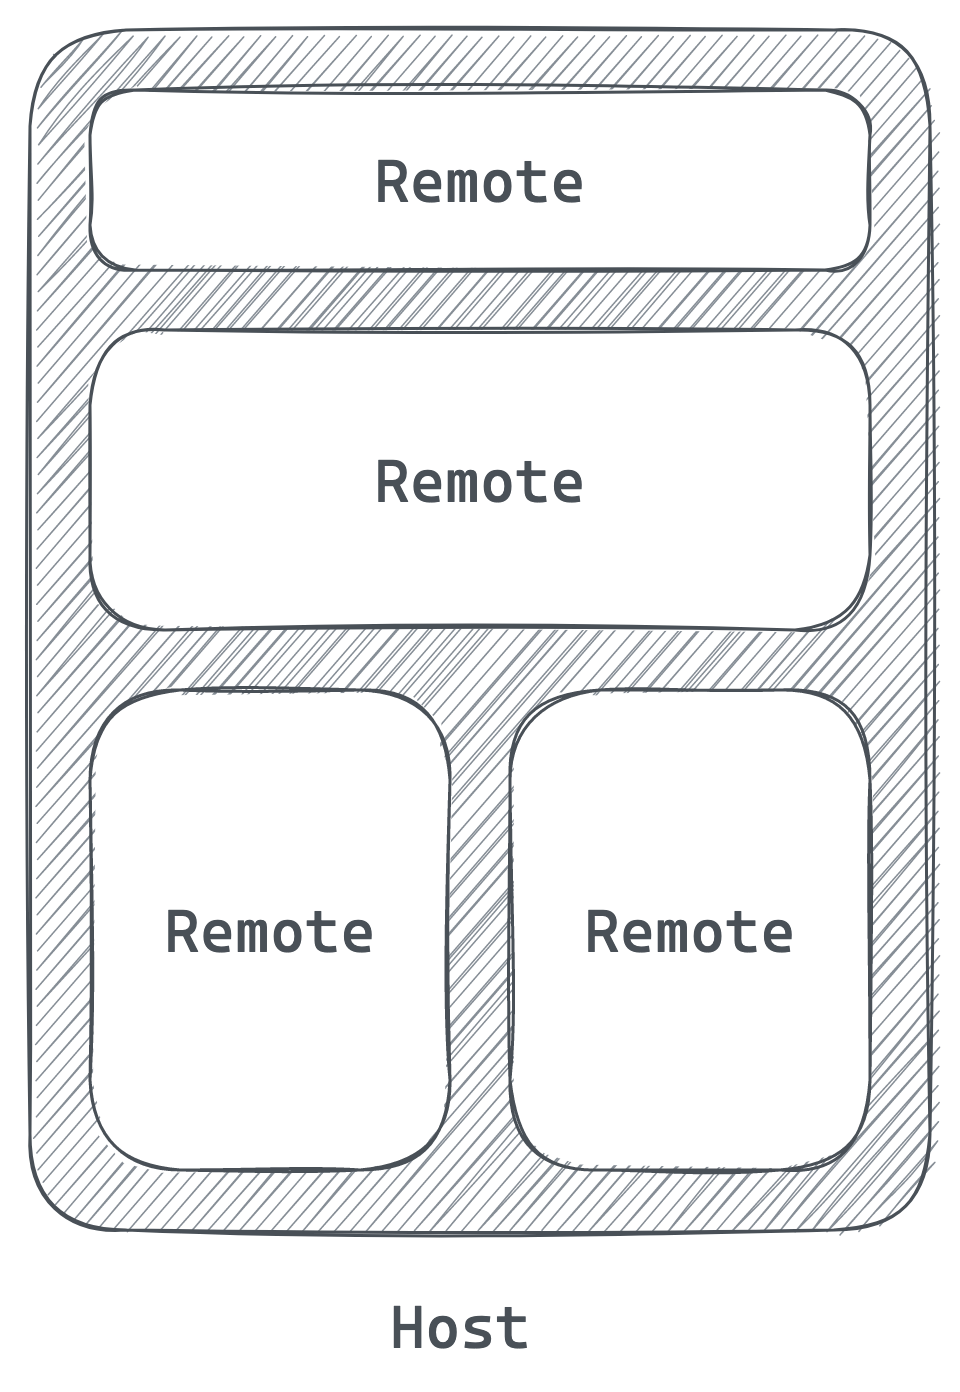
\includegraphics[width=0.3\linewidth]{images/module-federation-architecture.png}
    \caption{A prototypical micro-frontend architecture, that shows a host application that loads multiple remotes into the application. (Adapted from \cite[119]{book:2021:mezzalira:applied-methods:building-micro-frontends})
    }\label{fig:background:micro-frontend:module-federation:module-federation-architecture}
\end{figure}
\fi

Module Federation allows the code to be shared bidirectional, allowing a remote to share or the whole bundle with a host and vice versa. But bidirectional sharing can complicate the architecture quite easily. The best approach is to share only in one direction, so that the host never shares code with the remote. \cite[119]{book:2021:mezzalira:applied-methods:building-micro-frontends}

\subsubsection{Configuring Module Federation}

Configuring module federation is done inside the webpack configuration. Listing \ref{fig:background:micro-frontend:module-federation:configuring-module-federation} shows the configuration of the host application.

\ifshowListings
\begin{listing}[H]
    \begin{minted}{typescript}
plugins: [
  new ModuleFederationPlugin({
    name: 'Host',
    remotes: {
      Contact: 'Contact@http://localhost:4201/remoteEntry.js',
      Sales: 'Sales@http://localhost:4202/remoteEntry.js',
    }
    shared: [
      '@angular/core': {
        singleton: true,
      },
      '@angular/router': {
        singleton: true,
      },
      '@angular/material': {
        singleton: true,
      },
      ...
    ],
  }),
],
    \end{minted}
    \caption{Configuring Module Federation for the host application.}\label{fig:background:micro-frontend:module-federation:configuring-module-federation}
\end{listing}
\fi

\noindent First the name has to be defined, in this case \textbf{Host}. Inside the \textbf{remotes} object, we have to define the remote modules, that should be loadable into the host. Every remote consists of an ID and an associated URL where the remoteEntry.js, which contains a map of all JavaScript chunks for the micro-frontend that should be fetched. These two values are separated through an @ symbol. \cite[124]{book:2021:mezzalira:applied-methods:building-micro-frontends}

\noindent For example the contact micro-frontend has the ID \textit{Contact} and a local URL like \textit{http:\/\/localhost:4201\/remoteEntry.js}. This means that when the host loads the catalog micro-frontend, Module Federation will fetch the \textit{remoteEntry.js} file to understand, which JavaScript chunks should be loaded. And which dependencies should be shared. \cite[125]{book:2021:mezzalira:applied-methods:building-micro-frontends}

\noindent The \textbf{shared} array contains the libraries, which should be shared across all micro-frontends. With Module Federation, though, we just have to specify the dependencies we want to share in every remote and host. In our case, that's all the micro-frontends and the application shell. Then webpack and Module Federation will create multiple JavaScript files, downloading them only once for every user's session across all micro-frontends. \cite[125]{book:2021:mezzalira:applied-methods:building-micro-frontends}

\noindent As shown inside the \textbf{shared}-array in listing \ref{fig:background:micro-frontend:module-federation:configuring-module-federation}, a part of the libraries that should be shared is listed. How the dependencies are shared can be configured in many ways. The property \textbf{singleton} means that the library is only loaded once. Loading all shared library, before the application code is fetched is executed by using the \textbf{eager} property. With the \textit{requiredVersion} the version of the library can be configured. These are only some of the configuration properties are available, there exist many more. \cite[125]{book:2021:mezzalira:applied-methods:building-micro-frontends}

The dependencies that are exposed through Module Federation can be loaded synchronously or asynchronously through the \textit{eager} property. It is recommended to load the dependencies asynchronously, as the application can be loaded faster.
